\section{Matlab Application}
With all the mathematics behind the whole segmentation, feature extraction and classification parts, we realized that instead of having to manually manage each and every function, a more intuitive way of utilizing the whole setup was needed. This lead to the production of a graphical user interface (GUI) consisting of different elements the user could interact with in order to take a piece of sound, segment it and then get an automatic classification.

\subsection{Graphical User Interface}
Figure \ref{app-gui} shows the GUI of the active application, in which a waveform has been loaded segmented and annotated using the implemented kNN classifier. Starting from the top left corner (rectangle 1), we have a plot of the loaded signal. When this signal have been segmented, either automatically or manually, a set of vertical lines will be plotted to show the segmentation of the waveform. Along with the segmentation, the below plot (rectangle 3) will contain the change in the log-energy (log(RMS)), which should show a peak for each segment above. When the semgents have been classified, the results will be presented in the table (rectangle 6) with one cell for each segment. To load the unclassified signal into the application the user must choose one of two options: load a sound file or make a new recording. This is done in the top right of the GUI (rectangle 2). Pressing the "Load wave" button will present the user with a file dialog, so a sound file can be located somewhere on the machine. The "Start recording" and "Stop recording" buttons will turn on and off the microphone to receive some input. When the sound is loaded a playback button will play the sound for the user. Before the classification, the user must choose the features used in the process. On the middle right side of the GUI (rectangle 4) is where features can be checked and their analysis window size and skip can be adjusted. Finally, below the features (rectangle 5) the user can load a manually segmented (and annotated) dataset for the classifier. Pressing "Load train data" will prompt the user to choose a sound file first and then a text file containing the segmentation info (such as a segments start-point, duration and annotation). When the features above are chosen and adjusted the classifier can be trained using the "Train" button and finally the signal can be classified from the "Classify" button.

\begin{sidewaysfigure}
\begin{center}
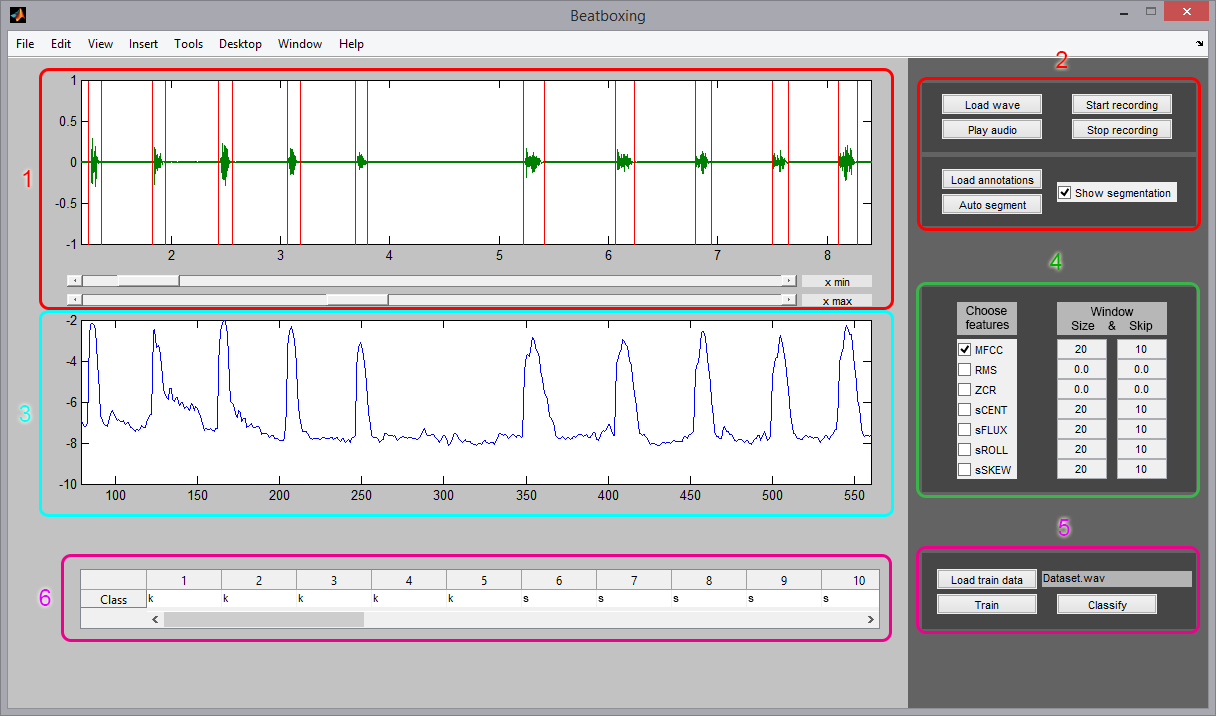
\includegraphics[width=\textwidth]{fig/Application.png}
\caption{Screenshot of the application GUI}
\label{app-gui}
\end{center}
\end{sidewaysfigure}

\subsection{Application Workflow}
When the user starts the application the flow has to follow a specific path from taking an unclassified signal, segment it and then automatically classify each sound included. The flow of the application is presented in figure \ref{app-flowchart}. To use the application the thing to do after starting it is to load a waveform of some recording of a person beatboxing, be it you or someone else. This waveform then has to be segmented to identify the points at which each beatboxing sound (e.g. a kick drum or hi-hat) starts and ends. This process can either be done manually by the user or it can automatically be done with the in-built segmentation algorithm. The manual process of segmenting the waveform has been explained in section \ref{sec:data-collection} about data collection using Sonic Visualiser. The automatic segmentation uses the implementation described above.

\begin{figure}
\begin{center}
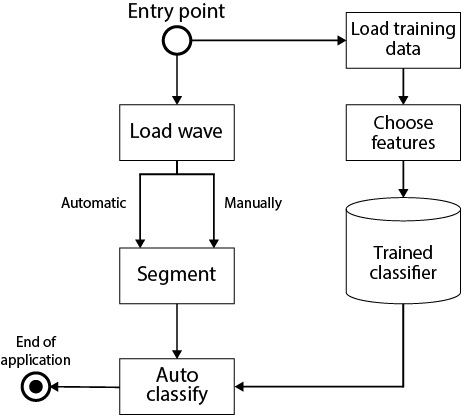
\includegraphics[scale=0.6]{fig/Application_flowchart.png}
\caption{Flowchart of the application.}
\label{app-flowchart}
\end{center}
\end{figure}

Before classifying these segments, the classifier has to be trained. To do this we start by loading a dataset that has been manually segmented. This dataset is a recording of multiple instances of the different beatboxing sounds used for the classification. When this dataset is loaded and segmented, the user must choose which features to use during the classification process. As an example we could choose MFCC using an analysis window size of 16 ms and a window skip of 8 ms. The classifier will then analyse all segments in the training dataset based on their MFCC and then store these analysis results to use them when classifying the unknown waveform.

When the user query a classification of the input waveform the classifier will take each segment from the input and compare it to the stored training data. Each segment will through this process get an annotation, i.e. a classification id, telling the user what kind of sound that segment has been interpreted as. A sequence of these annotation could be:

\begin{center}
k k k hh k s
\end{center}

, where the three first segments are classified as kicks followed by a hi-hat and then a snare.

Hereafter the user can try and adjust chosen features or choose new features to train the classifier again and/or a new waveform can be loaded into the application and segmented also to be classified.